\section{Protocolo de transmisión}
	\subsection{Descripción del problema}
	Desarrollar un programa que genere 50 cadenas de 32 caracteres que sean guardadas en un archivo, para después ser evaluadas por un autómata, en este caso el de paridad binaria y guardar las cadenas binarias validas en otro archivo, siguiendo el siguiente diagrama.
	\begin{figure}[H]
		\begin{center}
			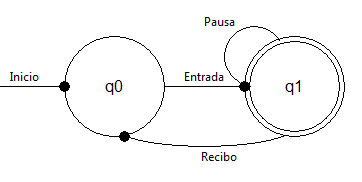
\includegraphics[width=10cm, height=5cm]{img/protocolo.png}
			\caption{Diagrama de transiciones del autómata. \cite{WEB}}
			\label{fig:diagrama3}
		\end{center}
	\end{figure}
	\subsection{Código}
	El código fue realizado en Python 3.5.
	\\Archivo: main\_protocolo.py
	\begin{lstlisting}[language=Python]
	#main_protocolo.py
	# -*- coding: utf-8 -*-
	from __future__ import print_function
	from diagrama_protocolo import Diagrama
	from protocolo import generar_cadenas, pausar_protocolo, verificar_cadenas
	import random
	
	separador = '*'*50
	
	def iniciar():
		continuar = True
		while continuar:
			opcion = imprimir_menu()
			if opcion == 1:
				correr_protocolo()
			elif opcion == 2:
				ver_diagrama()
			else:
				break # Sal del programa
			print('*' * 100)
			opcion = input("Reintentar s/n: ")
			if opcion.lower() != 's':
				continuar = False
		
		print('\nSaliendo del programa...')
	
	def imprimir_menu():
		print('\n\n%sMenu%s' % (separador, separador))
		print("""
		1.- Correr protocolo
		2.- Ver diagrama
		3.- Salir
		""")
		try:
			opcion = int(input("Selecciona una opcion valida: "))
			return opcion
		except Exception as e:
			print('Error ', e)
			return 0
	
	def correr_protocolo():
		condicion = True
		ARCHIVO_PALABRAS = 'palabras.txt'
		ARCHIVO_PALABRAS_VALIDAS = 'validas.txt'
		TIEMPO_PAUSA = 2
		palabras = []
		while condicion:
			archivo = open('validas.txt', 'w')
			print('\nGenerando cadenas...')
			generar_cadenas(ARCHIVO_PALABRAS)
			print('\nEnviando las candenas...')
			pausar_protocolo(TIEMPO_PAUSA)
			print('\nVerificando las cadenas las candenas...')
			verificar_cadenas(ARCHIVO_PALABRAS, palabras)
			print('\nRegresando las candenas...')
			print('\nPalabras validas: ', palabras)
			for palabra in palabras:
				archivo.write(palabra)
				archivo.write(' ')
			palabras = []
			condicion = random.choice([True, False])
			archivo.close()
	
	def ver_diagrama():
		print('Mostrando diagrama del automata. Cierre la ventana para continuar')
		try:
			diagrama_ere = Diagrama()
			diagrama_ere.master.title('Diagrama del protocolo')
			diagrama_ere.mainloop()
		except Exception as e:
			print("Error", e)
	
	iniciar()
	\end{lstlisting}
	Archivo: protocolo.py
	\begin{lstlisting}[language=Python]
	#protocolo.py
	# -*- coding: utf-8 -*-
	from __future__ import print_function
	import time, random
	
	def pausar_protocolo(segundos):
		time.sleep(segundos)
	
	def generar_cadenas(archivo):
		try:
			archivo_abierto = open(archivo, 'a')
		except Exception as e:
			print('Error al abrir archivo ', e)
		i = 0
		LONGITUD = 32
		numero_binario = ''
		
		for x in range(50):
			while i < LONGITUD:
				numero_binario += random.choice(['0', '1'])
				i += 1
			archivo_abierto.write(numero_binario)
			archivo_abierto.write(' ')
			i = 0
			numero_binario = ''
		
		archivo_abierto.close()
	
	def verificar_cadenas(archivo, palabras):
		try:
			archivo_abierto = open(archivo, 'r')
		except Exception as e:
			print('Error al abrir archivo ', e)
		
		texto = archivo_abierto.read()
		estado = 0
		palabra_aux = ''
		for simbolo in texto:
			print('-> delta(q%s,%s)' % (estado, simbolo), end="\t")
			
			if simbolo == ' ':
				if estado == 0:
					palabras.append(palabra_aux)
				palabra_aux = ''
				estado = 0
			else:
				palabra_aux += simbolo
				estado = automata(estado, simbolo)
		
	def automata(estado, simbolo):
		if estado == 0:
			estado = estado_cero(simbolo)
		elif estado == 1:
			estado = estado_uno(simbolo)
		elif estado == 2:
			estado = estado_dos(simbolo)
		elif estado == 3:
			estado = estado_tres(simbolo)
		else:
			print('Simbolo extrano ', simbolo)
			return -1
		return estado
	
	def estado_cero(simbolo):
		if simbolo == '0':
			return 2
		elif simbolo == '1':
			return 1
		else:
			return -1
	
	def estado_uno(simbolo):
		if simbolo == '0':
			return 3
		elif simbolo == '1':
			return 0
		else:
			return -1
	
	def estado_dos(simbolo):
		if simbolo == '0':
			return 0
		elif simbolo == '1':
			return 3
		else:
			return -1
	
	def estado_tres(simbolo):
		if simbolo == '0':
			return 1
		elif simbolo == '1':
			return 2
		else:
			return -1
	
	\end{lstlisting}
	Archivo: diagrama\_protocolo.py
	\begin{lstlisting}[language=Python]
	#diagrama_protocolo.py
	# -*- coding: utf-8 -*-
	from __future__ import print_function
	import tkinter as tk
	
	class Diagrama(tk.Frame):
		def __init__(self, master=None):
			super().__init__(master, background='white')
			self.pack(fill=tk.BOTH, expand=tk.YES)
			self.canvas = tk.Canvas(self, bg='white')
			self.canvas.pack(fill=tk.BOTH, expand=1)
			self.dibujarDiagrama()
			self.centrarVentana()
		
		def dibujarDiagrama(self):
			coordenadas = [70, 100, 170, 200]
			for x in range(2):
				self.escribirTexto(x, coordenadas)
				self.dibujarCirculo(coordenadas)
				self.dibujarFlecha([coordenadas[0]-80, 150, coordenadas[2]-100, 150])
				coordenadas[0] += 180
				coordenadas[2] += 180
		
			self.dibujarCirculo([coordenadas[0]-180+5, 105, coordenadas[2]-180-5, 195]) # circulo interior
			self.canvas.create_arc(230, 90, 290, 150, start=30, extent=235, style='arc')
			self.canvas.create_text(225, 85, text='Pausa')
			
			self.canvas.create_arc(120, 170, 300, 210, start=-30, extent=-120, style='arc')
			self.canvas.create_oval(130-5, 200-5, 130+5, 200+5, fill = 'black')
			self.canvas.create_text(225, 220, text='Recibo')
		
		def escribirTexto(self, x, coordenadas):
			text = ''
			text_flecha =''
			if x == 0:
				text = 'Listo'
				text_flecha = 'Inicio'
			elif x == 1:
				text = 'Enviando'
				text_flecha = 'Entrada'
			else:
				print('otro')
			
			self.canvas.create_text(coordenadas[0]+50, coordenadas[1]+50, font=('15'), text=text)
			self.canvas.create_text(coordenadas[0]-40, coordenadas[1]+40, text=text_flecha)
			
		def dibujarCirculo(self, arg):
			circulo = self.canvas.create_oval(arg)
		
		def dibujarFlecha(self, coordenadas):
			linea = self.canvas.create_line(coordenadas)
			self.canvas.create_oval(coordenadas[2]-5, coordenadas[1]-5, coordenadas[2]+5,coordenadas[1]+5, fill = 'black')
		
		def centrarVentana(self):
			ancho, altura = 400, 300
			ancho_pantalla = self.winfo_screenwidth()
			altura_pantalla = self.winfo_screenheight()
			posicion_x = (ancho_pantalla - ancho)/2
			posicion_y = (altura_pantalla - altura)/2
			self.master.geometry('%dx%d+%d+%d' % (ancho, altura, posicion_x, posicion_y))
	\end{lstlisting}
	
	\newpage
	\subsection{Pruebas}
	Pruebas de las opciones del menú.
	\\{\large Modo automático.}
	\begin{figure}[H]
		\begin{center}
			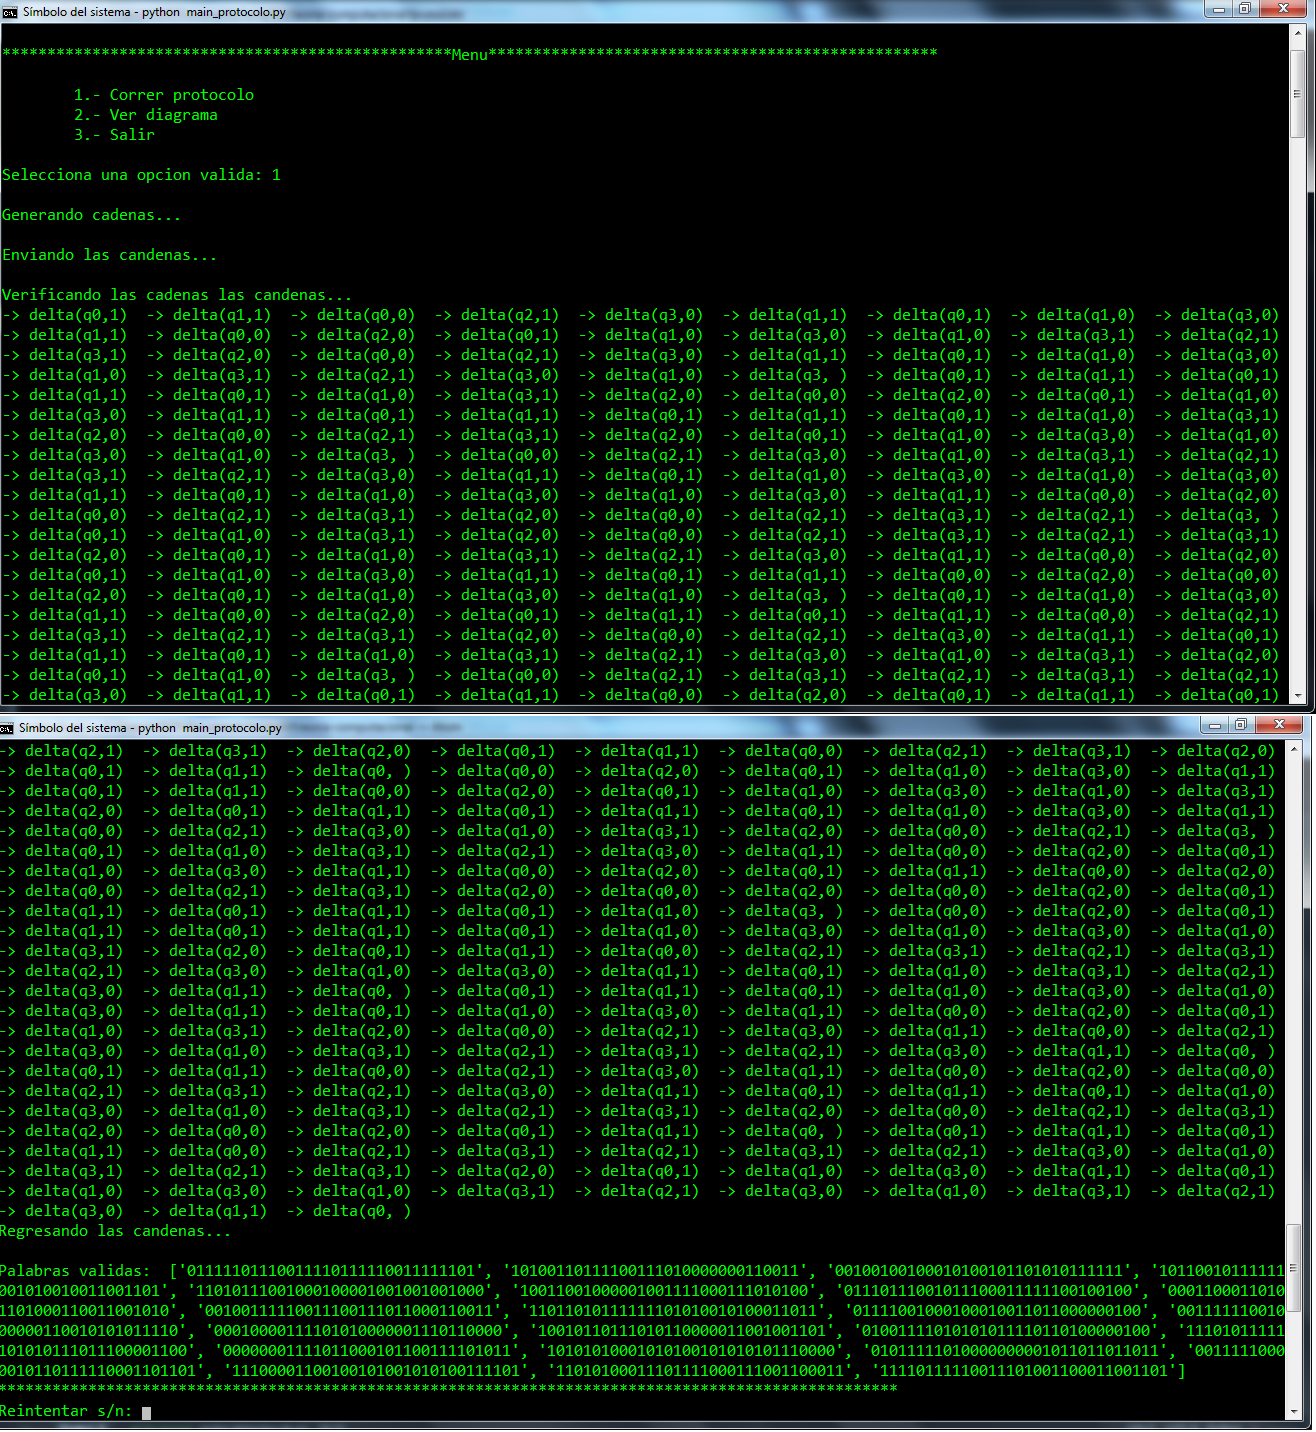
\includegraphics[width=\linewidth, height=15cm]{img/protocolo-automata.png}
			\caption{Parte de la historia del protocolo. \cite{WEB}}
			\label{fig:protocolo1}
		\end{center}
	\end{figure}
	\begin{figure}[H]
		\begin{center}
			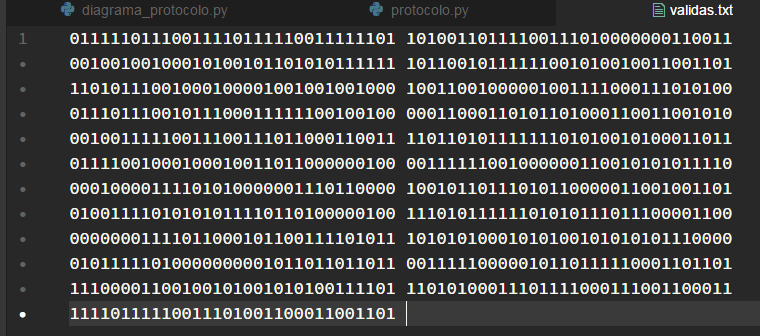
\includegraphics[width=\linewidth, height=5cm]{img/protocolo-salida.png}
			\caption{Palabras validas.\cite{WEB}}
			\label{fig:protocolo2}
		\end{center}
	\end{figure}
	{\large Diagrama.}
	\begin{figure}[H]
		\begin{center}
			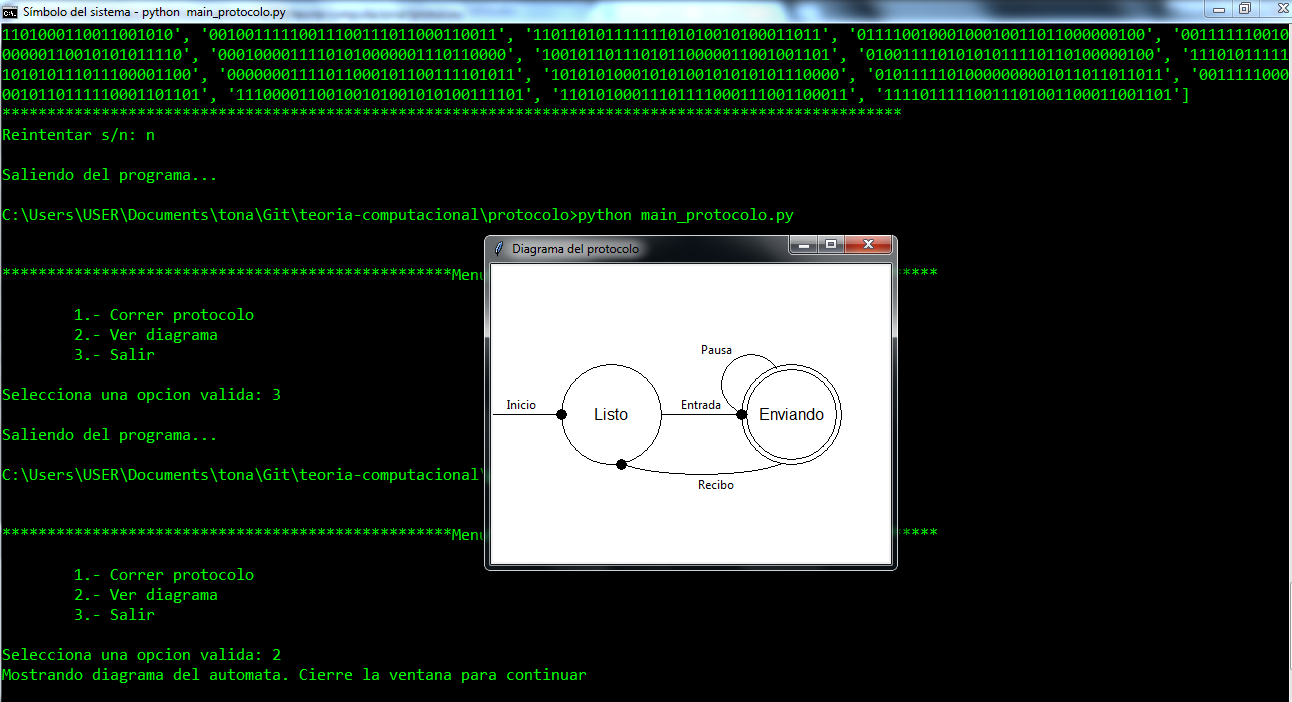
\includegraphics[width=\linewidth, height=10cm]{img/protocolo-diagrama.png}
			\caption{Diagrama de transiciones del autómata.}
			\label{fig:protocolo3}
		\end{center}
	\end{figure}